% ---------------------------------------------------------------------------
% Torre EV - Painel do Sindico
% Documentacao tecnica - Programacao de Dispositivos Moveis
%
% Compilar com pdflatex (duas passadas, por causa do sumario):
%     pdflatex Documentacao_TorreEV.tex
%     pdflatex Documentacao_TorreEV.tex
%
% As imagens ficam em ../includegraphics/ (ver \graphicspath abaixo).
% ---------------------------------------------------------------------------
\documentclass[12pt,a4paper]{article}

\usepackage[utf8]{inputenc}
\usepackage[T1]{fontenc}
\usepackage[brazil]{babel}
\usepackage{lmodern}

\usepackage[margin=2.5cm]{geometry}
\usepackage{graphicx}
\usepackage{pdflscape}
\usepackage{booktabs}
\usepackage{xcolor}
\usepackage{float}
\usepackage[font=small,labelfont=bf]{caption}
\usepackage{enumitem}
\usepackage[hidelinks]{hyperref}

\graphicspath{{../includegraphics/}}

\definecolor{azulapp}{HTML}{0D47A1}
\definecolor{cinzabox}{HTML}{F5F5F5}

\newcommand{\comp}[1]{\texttt{#1}}

\title{\vspace{-1.5cm}\textbf{Torre EV --- Painel do Síndico}\\[0.3cm]
\large Gestão de recarga de veículos elétricos em condomínio}
\author{Henrique Marangoni \and \textit{[nome do colega]}}
\date{Programação de Dispositivos Móveis \\ MIT App Inventor 2 \\[0.3cm] \today}

\begin{document}

\maketitle
\thispagestyle{empty}

\begin{center}
\begin{minipage}{0.85\textwidth}
\small
\textbf{Resumo.} O Torre EV é um painel de controle para o síndico acompanhar, em tempo
real, a recarga de veículos elétricos na garagem comum de um condomínio antigo. O
aplicativo soma a potência das recargas em andamento, compara com o limite elétrico do
prédio, alerta por texto e por voz quando a carga se aproxima do limite, recusa recargas
que o estourariam e registra o consumo em kWh por morador. Foi desenvolvido no MIT App
Inventor 2 e não exige nenhuma obra na rede elétrica existente.
\end{minipage}
\end{center}

\vspace{0.8cm}
\tableofcontents
\newpage

% ===========================================================================
\section{Definição do problema}

\subsection{O cenário}

O Residencial Parque das Torres foi construído no início dos anos 2000. São duas torres,
120 apartamentos e 240 vagas de garagem. A rede elétrica foi dimensionada há duas décadas
prevendo apenas iluminação das áreas comuns, portões eletrônicos e elevadores.

Recentemente, 15 moradores adquiriram veículos elétricos, e a expectativa é que esse
número dobre nos próximos meses. A tentativa inicial de ligar carregadores portáteis nas
tomadas comuns da garagem resultou em queda de disjuntores gerais, aumento
desproporcional na conta de energia da área comum e atrito entre vizinhos.

O problema não é falta de tomada. É que \textbf{ninguém consegue enxergar quanto está
sendo puxado da rede em cada momento}. O síndico só descobre que passou do limite quando
o disjuntor cai --- ou seja, depois do estrago.

\subsection{As dores, por ator}

\begin{table}[H]
\centering
\small
\begin{tabular}{@{}p{3.2cm}p{10.5cm}@{}}
\toprule
\textbf{Ator} & \textbf{Dor} \\
\midrule
Donos de veículo elétrico &
Insegurança na recarga; falta de previsibilidade sobre quanto tempo o carro precisa ficar
plugado; vontade de pagar exatamente pelo que consumiram. \\
\addlinespace
Síndico e administração &
Risco de sobrecarga no barramento principal, com potencial de incêndio ou interrupção do
fornecimento aos elevadores; impossibilidade de saber quanto cada morador consumiu;
mediação constante de conflitos. \\
\addlinespace
Moradores sem veículo elétrico &
Resistência a custear, via taxa condominial, a energia dos vizinhos; incômodo com cabos
espalhados pelas áreas de circulação. \\
\bottomrule
\end{tabular}
\caption{Dores identificadas no estudo de caso.}
\end{table}

\subsection{O nicho escolhido e o usuário final}

Seguindo a orientação do desafio de \textit{não} tentar resolver todo o ecossistema em um
único sistema, a equipe escolheu atacar as duas dores do bloco central da tabela:
\textbf{risco na infraestrutura} e \textbf{gestão de custos}.

\begin{quote}
\textbf{Usuário final: o síndico.} Não o motorista, não o morador sem carro elétrico. É o
síndico quem abre o aplicativo, cadastra as recargas em andamento e responde pela
integridade da rede elétrica do prédio.
\end{quote}

É importante registrar o que o aplicativo \textbf{não} é: ele não mede eletricidade. Não
há sensor nem medidor. O síndico informa quem plugou o carro e com que potência, e dá
baixa quando a recarga termina. O valor do sistema não está em medir, e sim em
\textbf{somar, avisar antes do estrago e registrar o consumo} --- transformando anotação
solta em decisão informada.

% ===========================================================================
\section{Visão geral da solução}

\subsection{A regra do semáforo}

O coração do aplicativo é uma classificação em três estados, recalculada automaticamente a
cada dois segundos:

\begin{table}[H]
\centering
\small
\begin{tabular}{@{}llp{7.2cm}@{}}
\toprule
\textbf{Estado} & \textbf{Condição} & \textbf{Resposta do aplicativo} \\
\midrule
Verde    & total $<$ 80\% do limite & Cartão verde, sem alerta \\
Amarelo  & total $\geq$ 80\% do limite & Cartão amarelo e aviso por voz \\
Vermelho & total $>$ limite & Cartão vermelho, notificação na tela e aviso por voz \\
\bottomrule
\end{tabular}
\caption{Regra de classificação da carga do barramento.}
\end{table}

A faixa amarela é o ponto central da proposta. O vermelho já é tarde: corresponde ao
disjuntor prestes a cair. O amarelo é o aviso que o síndico nunca teve.

\subsection{Navegação entre telas}

\begin{table}[H]
\centering
\small
\begin{tabular}{@{}llp{6.8cm}@{}}
\toprule
\textbf{Tela} & \textbf{Nome no projeto} & \textbf{Função} \\
\midrule
1 & \comp{Screen1}   & Login do síndico \\
2 & \comp{Painel}    & Dashboard: status, carga, limite, ações \\
3 & \comp{Cadastro}  & Registro de uma nova recarga \\
4 & \comp{Historico} & Recargas encerradas e consumo por morador \\
\bottomrule
\end{tabular}
\caption{As quatro telas do aplicativo.}
\end{table}

O fluxo é \comp{Screen1} $\rightarrow$ \comp{Painel}, e do painel partem e retornam
\comp{Cadastro} e \comp{Historico}. O painel é o centro da aplicação.

\subsection{Persistência: o que o TinyDB guarda}

Todo o estado do aplicativo vive no componente \comp{BancoLocal}, um \comp{TinyDB} presente
nas quatro telas. Ele grava pares tag--valor no próprio aparelho, e os dados sobrevivem ao
fechamento do aplicativo.

\begin{table}[H]
\centering
\small
\begin{tabular}{@{}llp{7.2cm}@{}}
\toprule
\textbf{Tag} & \textbf{Padrão} & \textbf{Conteúdo} \\
\midrule
\comp{senha}          & \comp{"1234"} & Senha do síndico \\
\comp{limiteKw}       & \comp{22}     & Limite elétrico destinado às recargas \\
\comp{recargasAtivas} & lista vazia   & Lista de \comp{[nome, kW, início]} em andamento \\
\comp{historico}      & lista vazia   & Lista de \comp{[nome, kWh, horas, data]} encerradas \\
\bottomrule
\end{tabular}
\caption{Estrutura de dados no TinyDB.}
\end{table}

\begin{quote}
\small
\textbf{Nota sobre o limite de 22 kW.} O enunciado do desafio descreve o condomínio (120
apartamentos, 240 vagas, 15 veículos elétricos) mas não informa a capacidade elétrica
disponível. O valor de 22~kW é, portanto, uma \textbf{decisão de projeto} da equipe, e não
um dado do estudo de caso. Como o limite é ajustável em tempo de execução pelo próprio
síndico, o aplicativo se adapta a qualquer capacidade real que venha a ser medida.
\end{quote}

\begin{quote}
\small
\textbf{Nota sobre o tipo dos dados.} O horário de início é gravado em milissegundos
(número), e não como objeto de data. O TinyDB persiste apenas texto, número, booleano e
lista; um objeto de data é serializado por sua representação textual e volta como texto,
inutilizável para cálculo. A duração é obtida por subtração de milissegundos.
\end{quote}

% ===========================================================================
\section{Telas da solução}

\subsection{Tela 1 --- Login}

Protege o painel com a senha do síndico, lida do TinyDB. O campo tem a propriedade
\comp{Password} ativada, mascarando a digitação.

\begin{figure}[H]
\centering
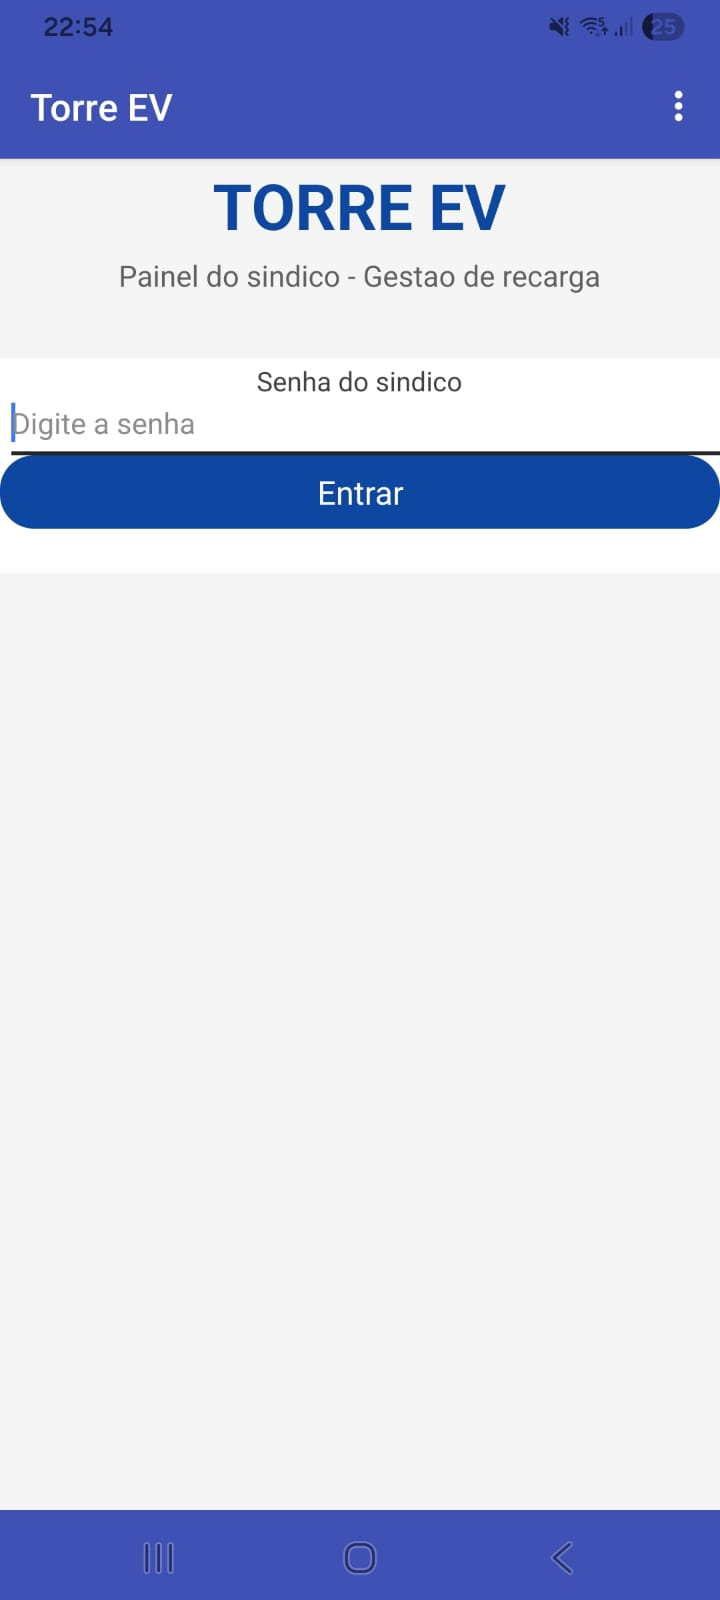
\includegraphics[height=0.42\textheight]{print-tela-inicial.jpg}
\caption{Tela de login. A senha padrão é \comp{1234} e fica armazenada no TinyDB, podendo
ser alterada sem recompilar o aplicativo.}
\end{figure}

\subsection{Tela 2 --- Painel}

Concentra toda a informação de operação: estado atual, carga em kW, limite vigente,
número de vagas em uso e as três ações disponíveis. Atualiza-se sozinha a cada dois
segundos.

\begin{figure}[H]
\centering
\begin{minipage}{0.47\textwidth}
\centering
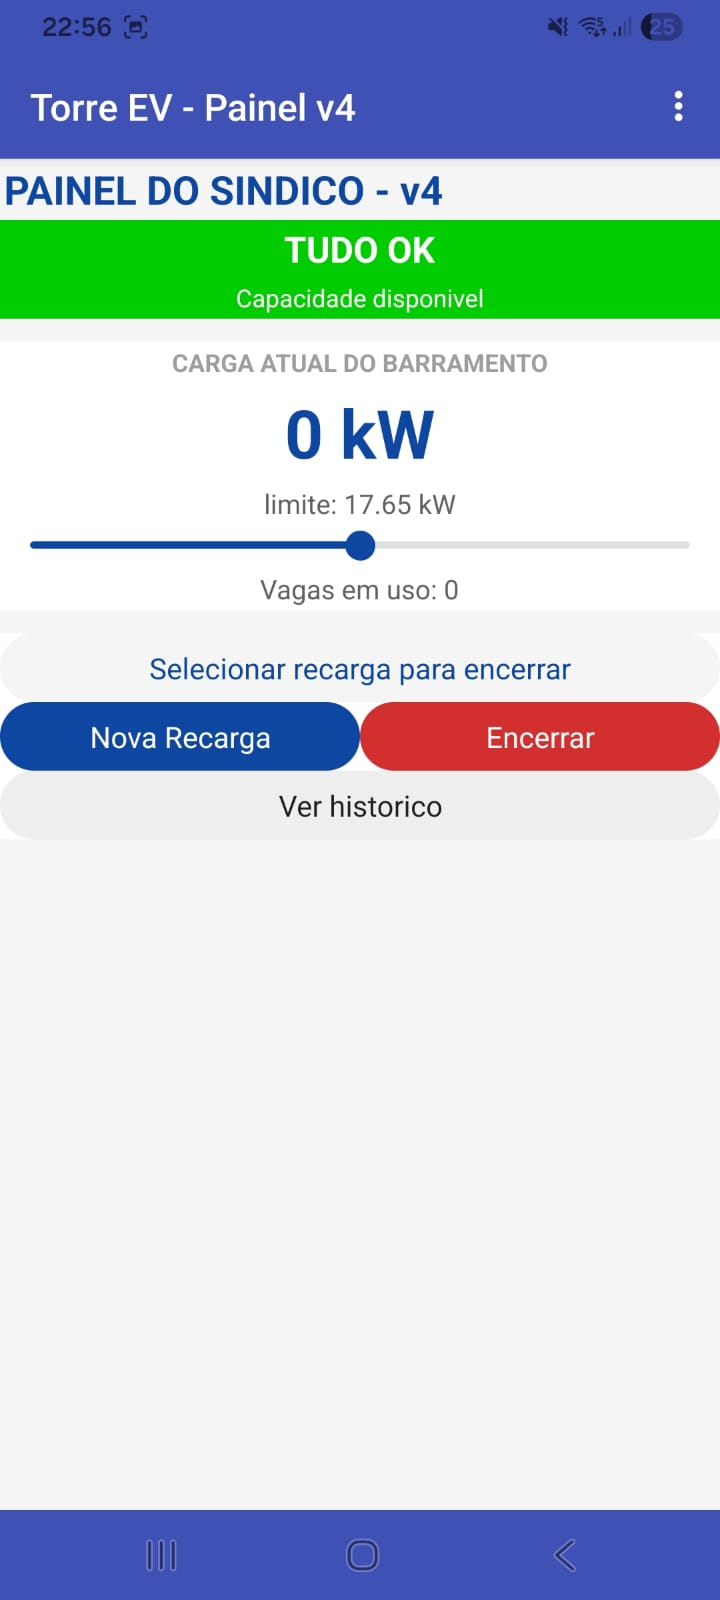
\includegraphics[height=0.42\textheight]{print-painel-verde.jpg}
\end{minipage}\hfill
\begin{minipage}{0.47\textwidth}
\centering
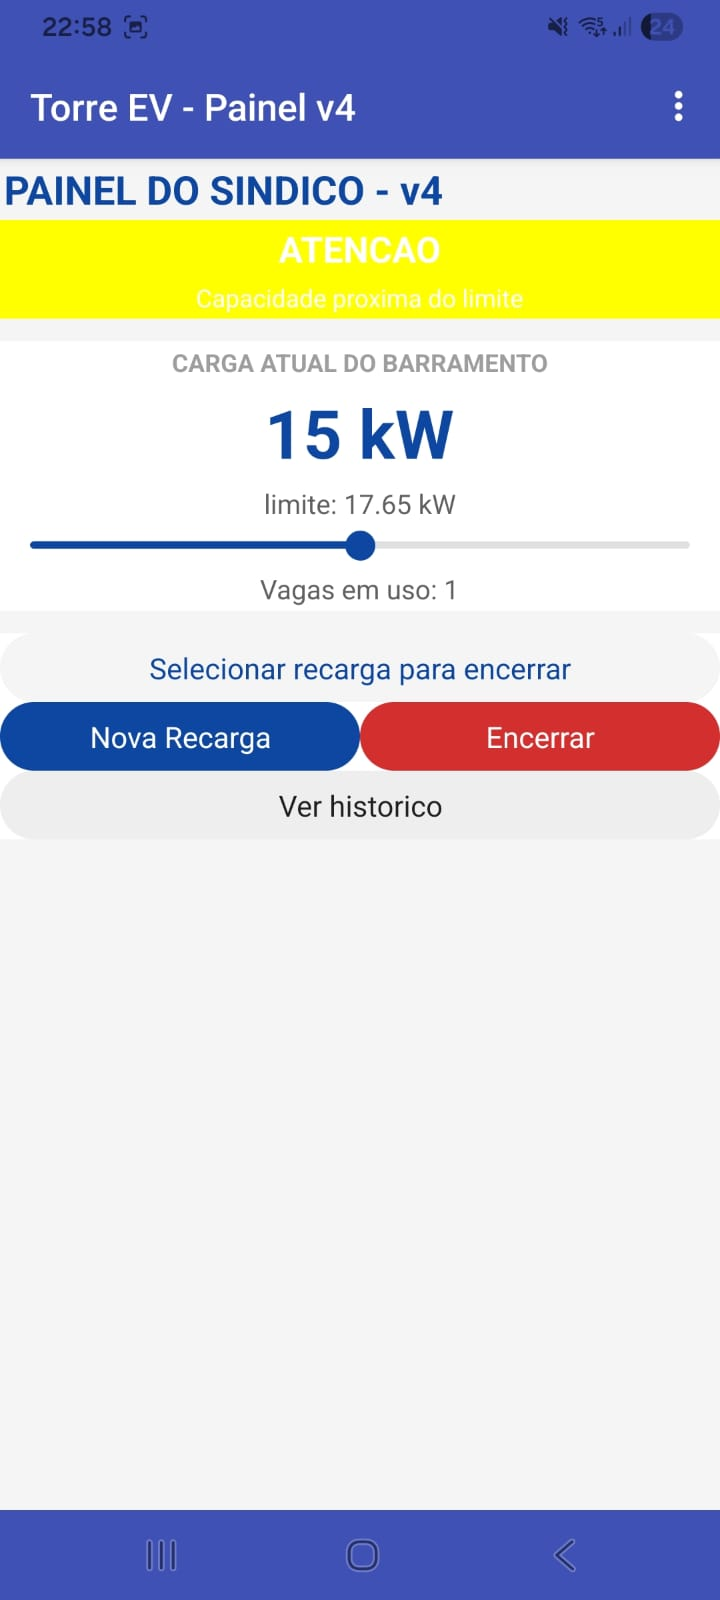
\includegraphics[height=0.42\textheight]{print-painel-amarelo.jpg}
\end{minipage}
\caption{Painel em dois estados. À esquerda, carga folgada (verde). À direita, carga acima
de 80\% do limite (amarelo), situação em que o aplicativo também emite aviso por voz.
A barra deslizante sob o valor de carga é o controle do limite, ajustável de 5 a 60~kW.}
\end{figure}

\begin{figure}[H]
\centering
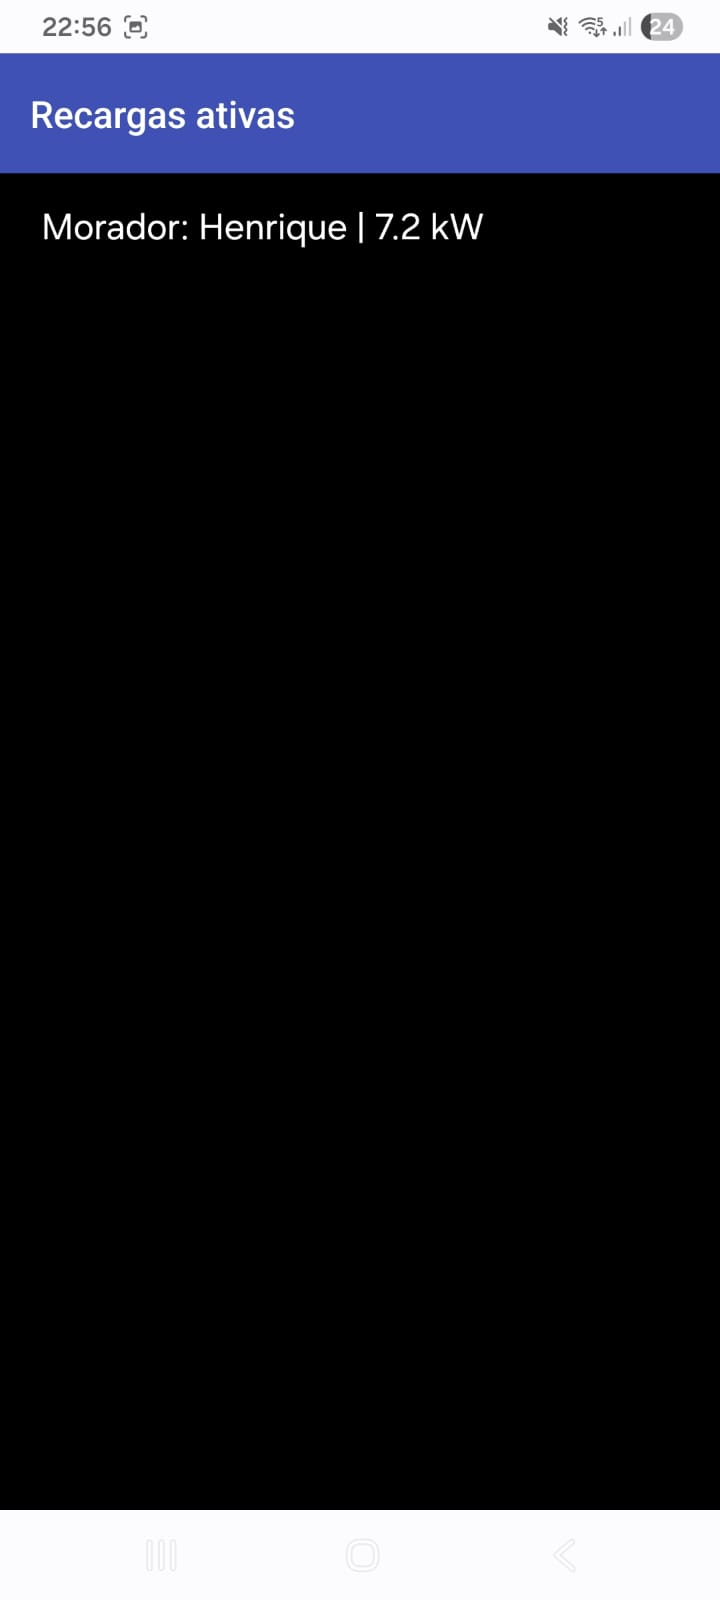
\includegraphics[height=0.40\textheight]{print-recargas-ativas.jpg}
\caption{Seleção da recarga a encerrar. A lista é montada a partir das recargas ativas
gravadas no TinyDB e mostra o morador e a potência de cada uma.}
\end{figure}

\subsection{Tela 3 --- Cadastro de recarga}

Recebe o nome do morador e a potência do carregador. O campo de potência aceita ponto ou
vírgula como separador decimal, e a validação ocorre no momento de salvar.

\begin{figure}[H]
\centering
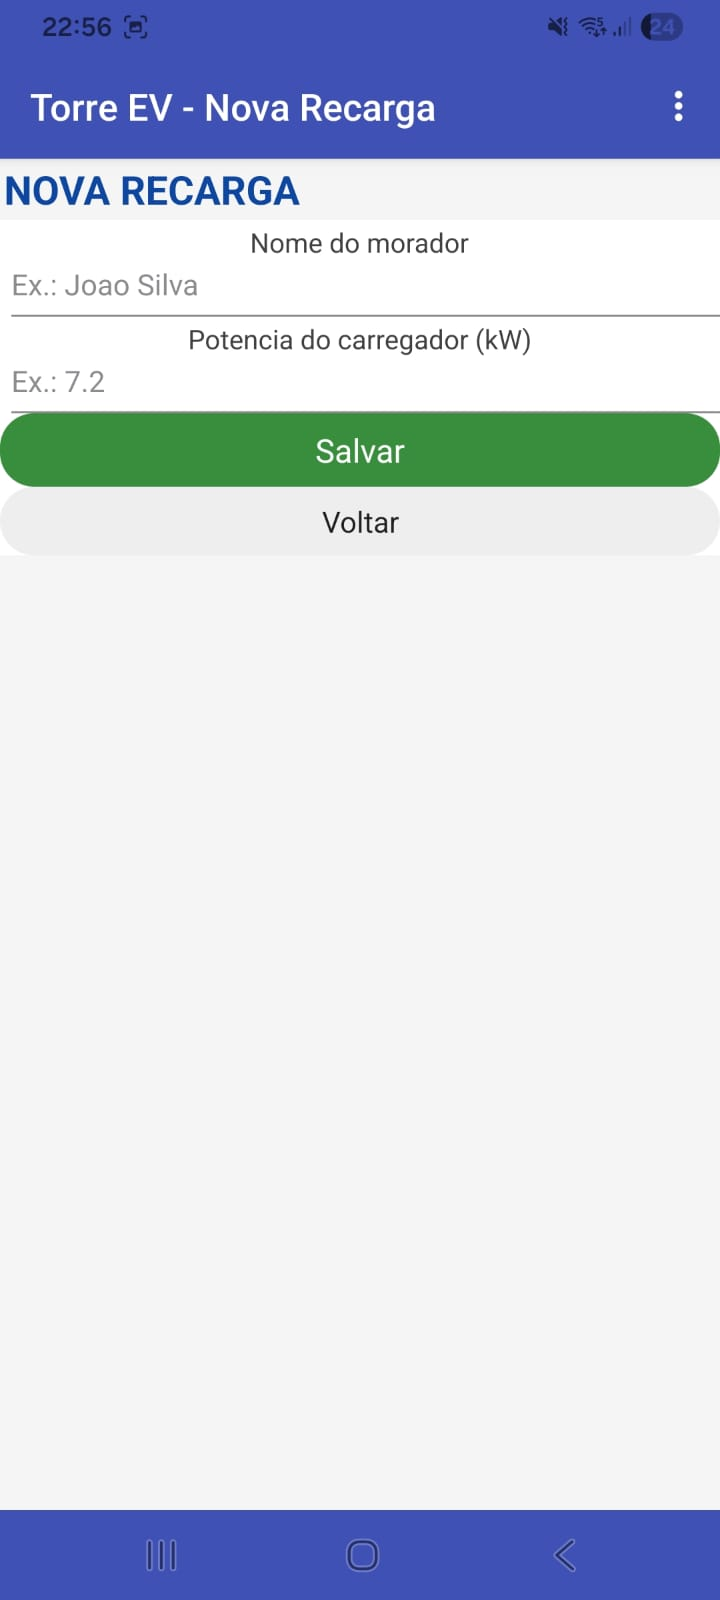
\includegraphics[height=0.42\textheight]{print-nova-recarga.jpg}
\caption{Tela de cadastro. Os textos de exemplo (\textit{hints}) orientam o formato
esperado em cada campo.}
\end{figure}

\subsection{Tela 4 --- Histórico}

Lista as recargas já encerradas. Cada linha traz cinco informações: morador, energia
consumida, duração, potência do carregador e o instante do encerramento.

\begin{figure}[H]
\centering
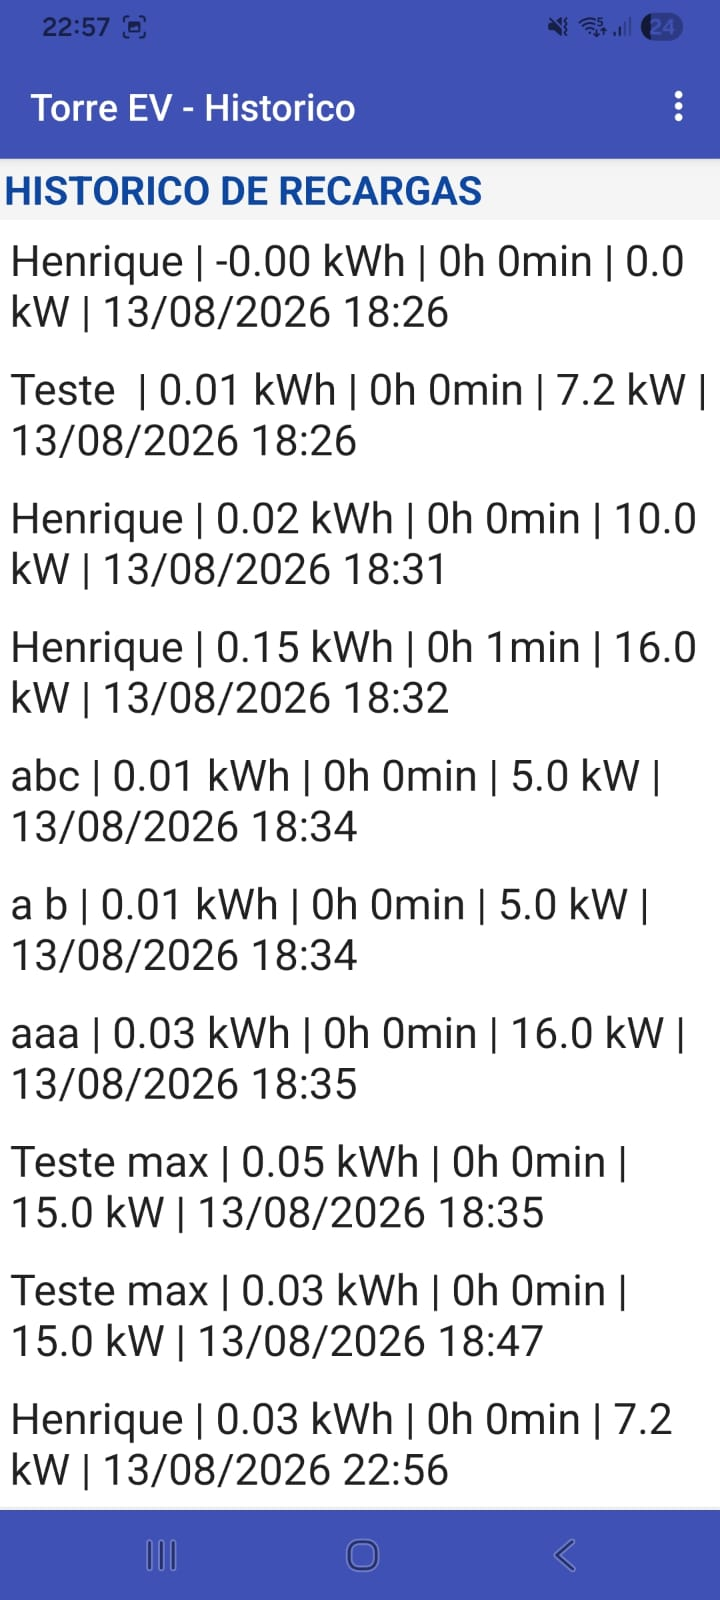
\includegraphics[height=0.44\textheight]{print-historico.jpg}
\caption{Histórico de recargas encerradas. A potência exibida é derivada da razão entre
energia e duração, e não de um campo adicional --- decisão que mantém compatibilidade com
registros gravados por versões anteriores do aplicativo.}
\end{figure}

% ===========================================================================
\section{Diagrama de blocos e algoritmo}

Esta seção percorre a lógica do aplicativo, com ênfase nas estruturas condicionais
encadeadas e no uso do TinyDB, conforme pedido no enunciado.

\subsection{Login: validação de senha}

\begin{figure}[H]
\centering
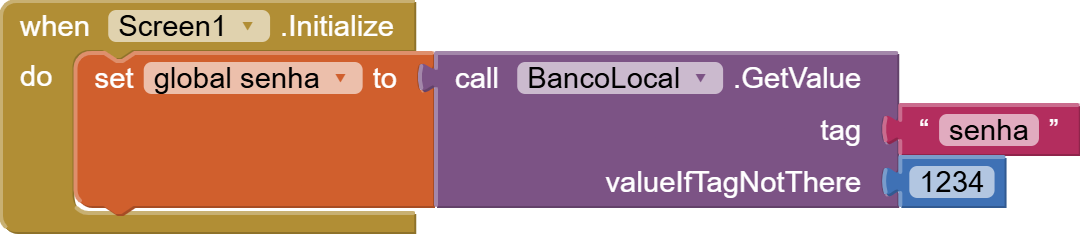
\includegraphics[width=0.85\textwidth]{login-inicializa.png}
\caption{\comp{Screen1.Initialize}. Ao abrir o aplicativo pela primeira vez, o TinyDB
ainda não tem a tag \comp{senha}; o segundo argumento de \comp{GetValue} fornece o valor
padrão \comp{1234}, que é então gravado. Nas execuções seguintes o valor lido é o que
estiver armazenado.}
\end{figure}

\begin{figure}[H]
\centering
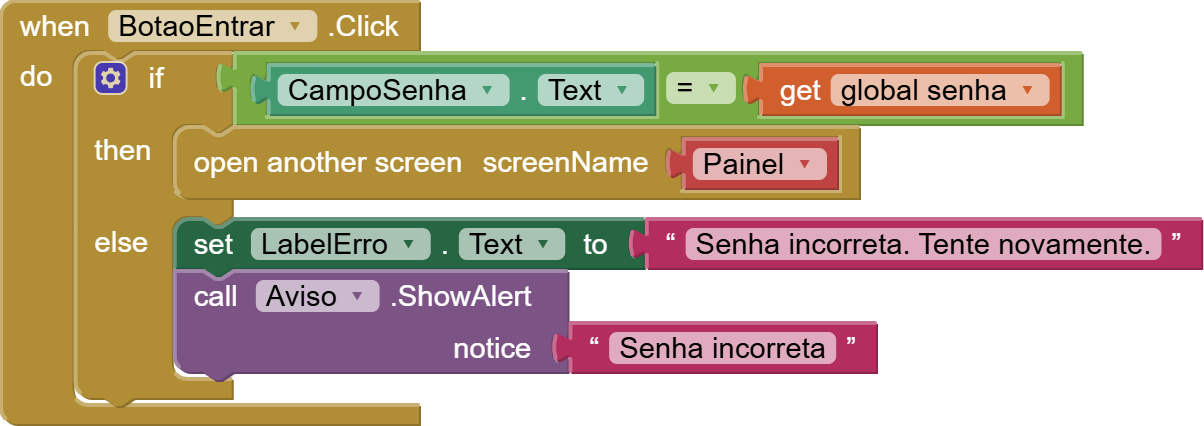
\includegraphics[width=0.95\textwidth]{login-entrar.png}
\caption{\comp{BotaoEntrar.Click}. Condicional simples: se o texto digitado for igual à
senha armazenada, abre o painel; caso contrário, escreve a mensagem de erro no rótulo
\comp{LabelErro} e permanece na tela.}
\end{figure}

\subsection{Painel: inicialização e atualização automática}

\begin{figure}[H]
\centering
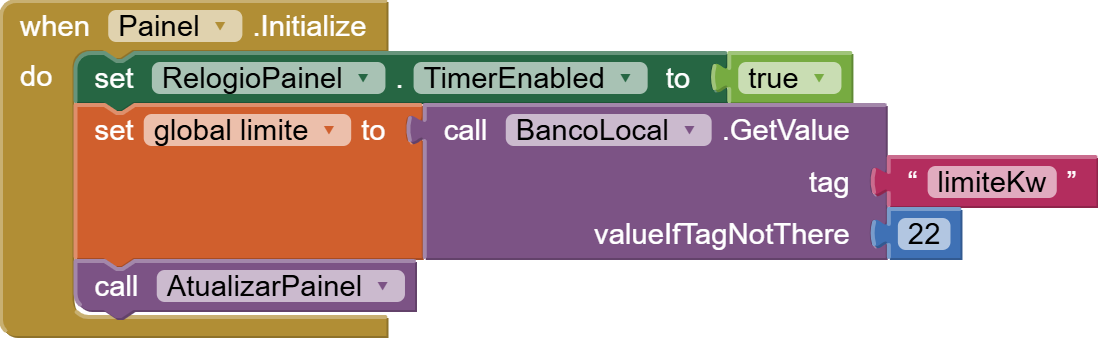
\includegraphics[width=0.9\textwidth]{painel-inicializa.png}
\caption{\comp{Painel.Initialize}. Liga o temporizador, carrega o limite gravado no TinyDB
(com 22~kW como padrão), posiciona a barra deslizante no valor carregado e faz a primeira
atualização do painel.}
\end{figure}

\begin{figure}[H]
\centering
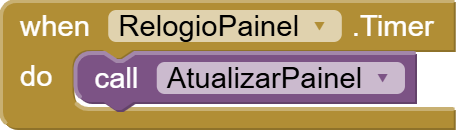
\includegraphics[width=0.55\textwidth]{painel-timer.png}
\caption{\comp{RelogioPainel.Timer}. A cada 2000~ms o procedimento \comp{AtualizarPainel}
é executado. É isso que torna o painel um monitor, e não uma tela estática.}
\end{figure}

\begin{figure}[H]
\centering
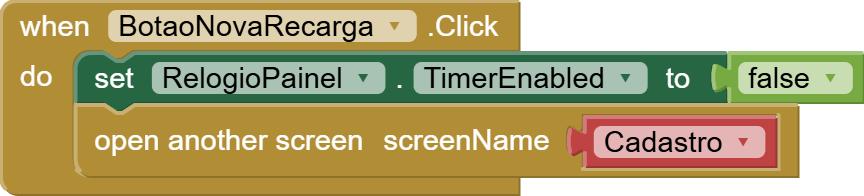
\includegraphics[width=0.75\textwidth]{painel-abre-cadastro.png}
\caption{\comp{BotaoNovaRecarga.Click}. O temporizador é \textbf{desligado} antes de abrir
outra tela. Sem isso, o procedimento do painel continuaria sendo disparado enquanto outra
tela estivesse em primeiro plano, tentando escrever em rótulos que não existem naquele
contexto.}
\end{figure}

\begin{figure}[H]
\centering
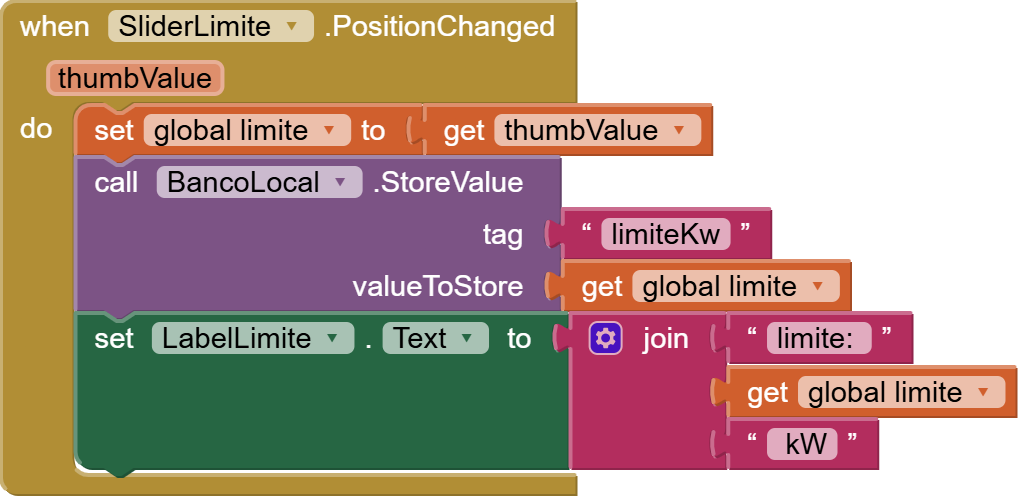
\includegraphics[width=0.9\textwidth]{painel-slider.png}
\caption{\comp{SliderLimite.PositionChanged}. Ao arrastar a barra, o novo valor vira o
limite corrente, é gravado no TinyDB e refletido no rótulo. A próxima execução de
\comp{AtualizarPainel} já reavalia o semáforo contra o limite novo.}
\end{figure}

\subsubsection{O procedimento \texorpdfstring{\comp{AtualizarPainel}}{AtualizarPainel}}

É o bloco central do aplicativo (Figura~\ref{fig:atualiza}). O algoritmo é:

\begin{enumerate}[itemsep=2pt]
\item Zera o acumulador \comp{total} e a lista \comp{nomes}.
\item Percorre \comp{recargasAtivas}, lida do TinyDB, somando a potência de cada recarga
      e montando a descrição que aparecerá no seletor.
\item Escreve nos rótulos de carga, limite e vagas em uso.
\item Atualiza o seletor \textbf{apenas se a lista de nomes mudou}, comparando com
      \comp{nomesAnt}. Sem essa comparação, a seleção feita pelo síndico seria descartada
      a cada dois segundos.
\item Classifica a carga em uma \textbf{condicional encadeada de três ramos}:
      \texttt{se} total $>$ limite, \texttt{senão se} total $>$ 80\% do limite,
      \texttt{senão} normal.
\item Dentro de cada ramo, uma segunda condicional compara o estado atual com
      \comp{statusAnt}. Cor e textos são reescritos, e o alerta sonoro é disparado,
      \textbf{apenas na transição} de estado. É isso que impede o aplicativo de repetir o
      mesmo aviso a cada dois segundos.
\end{enumerate}

\begin{figure}[p]
\centering
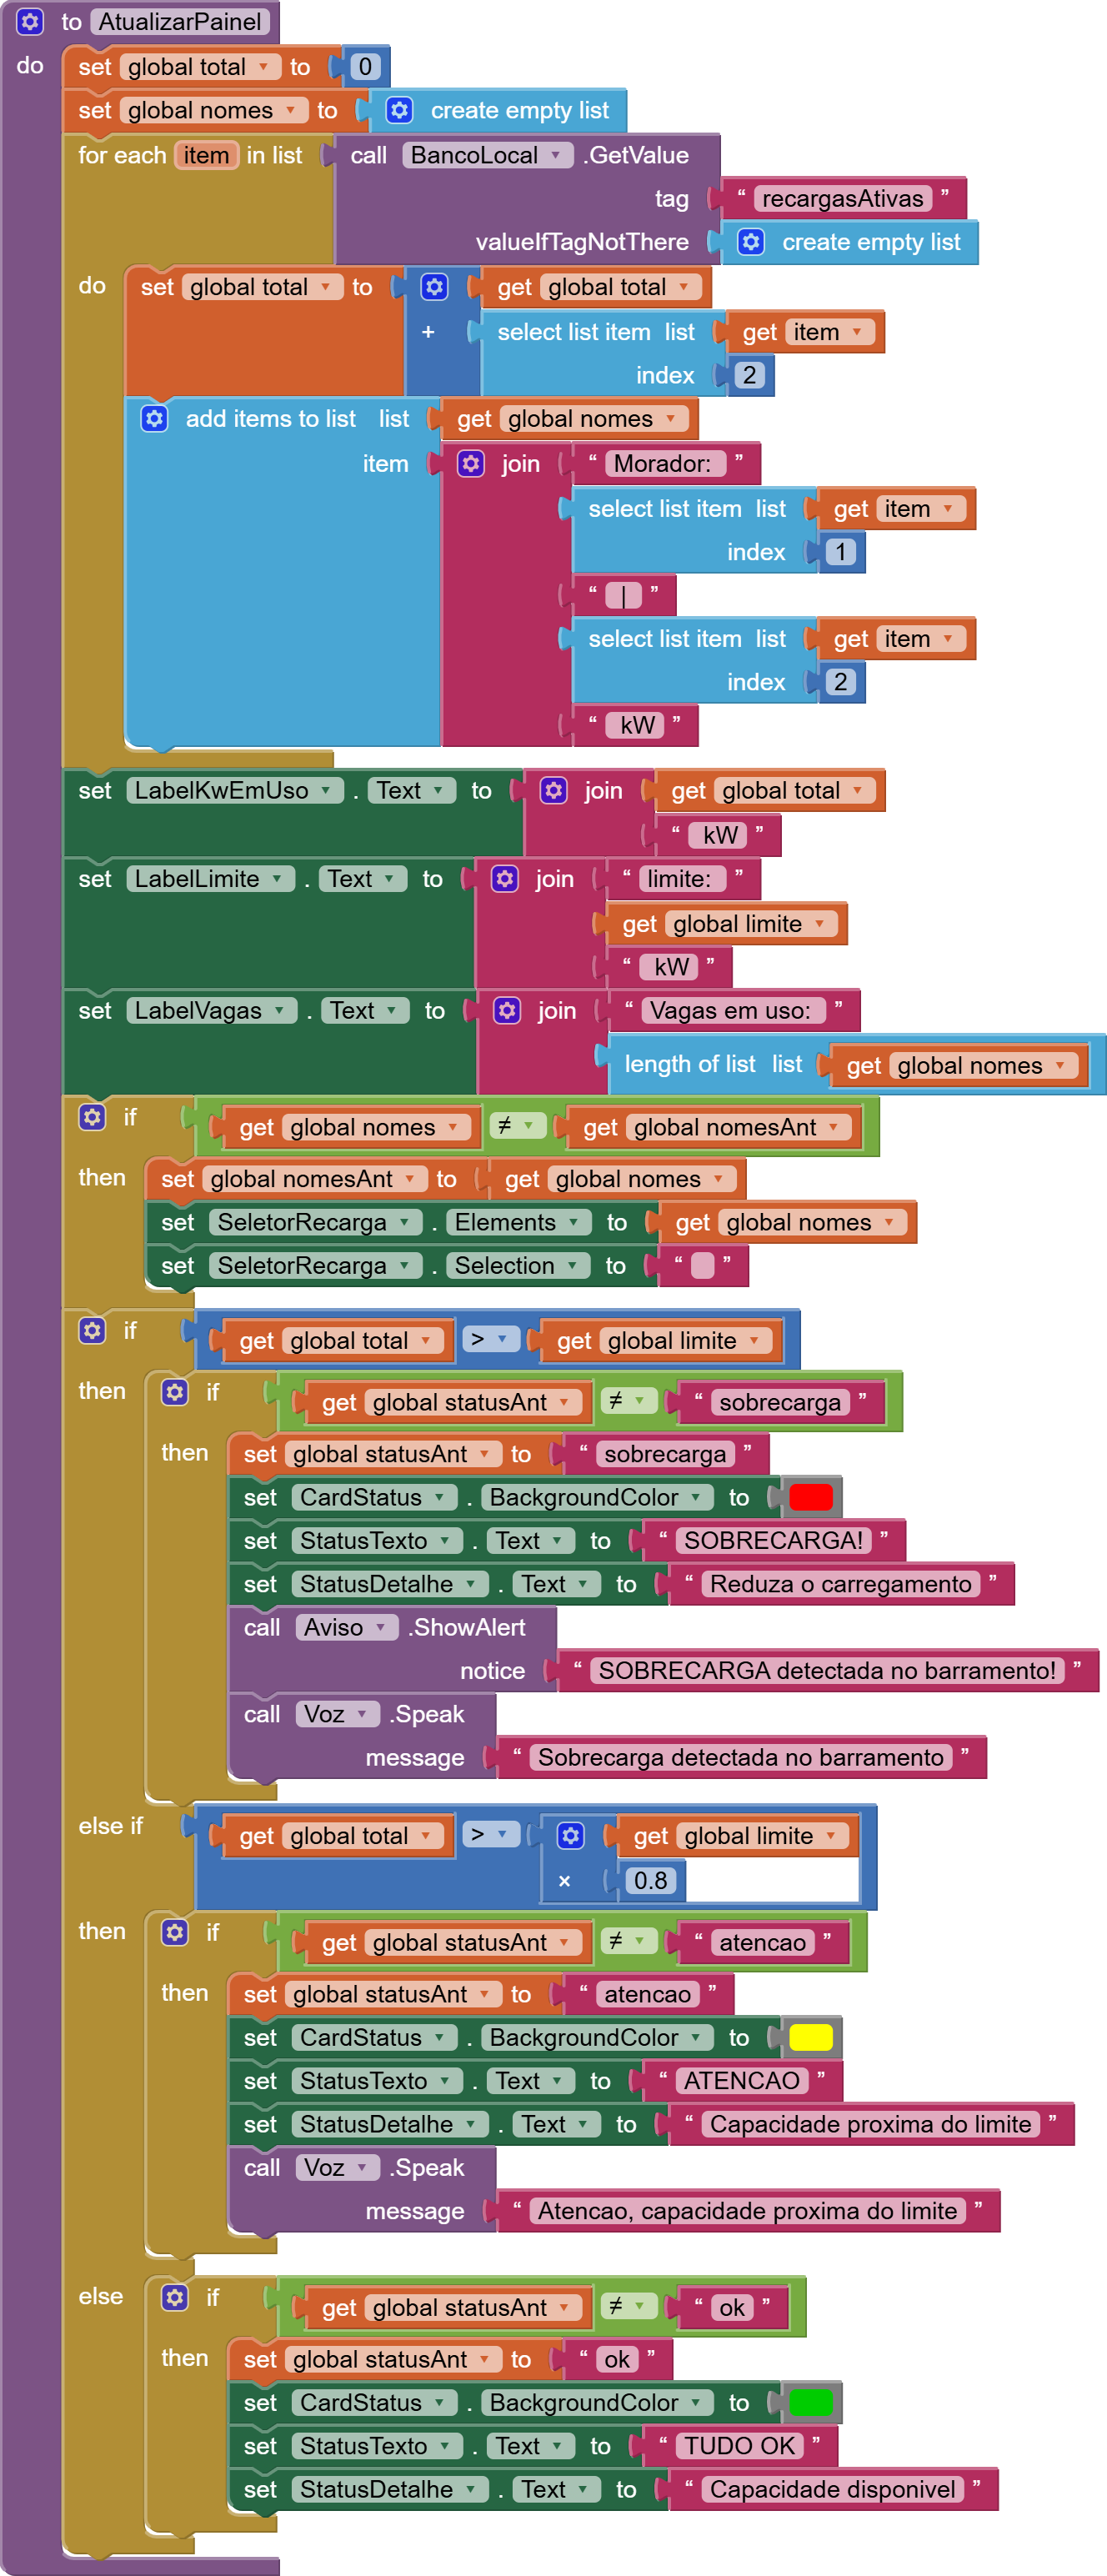
\includegraphics[height=0.92\textheight]{painel-atualiza.png}
\caption{Procedimento \comp{AtualizarPainel}, executado a cada dois segundos. A condicional
externa classifica a carga; as internas garantem que o alerta ocorra somente na mudança de
estado.}
\label{fig:atualiza}
\end{figure}

\subsubsection{Encerramento e cálculo de consumo}

\begin{figure}[H]
\centering
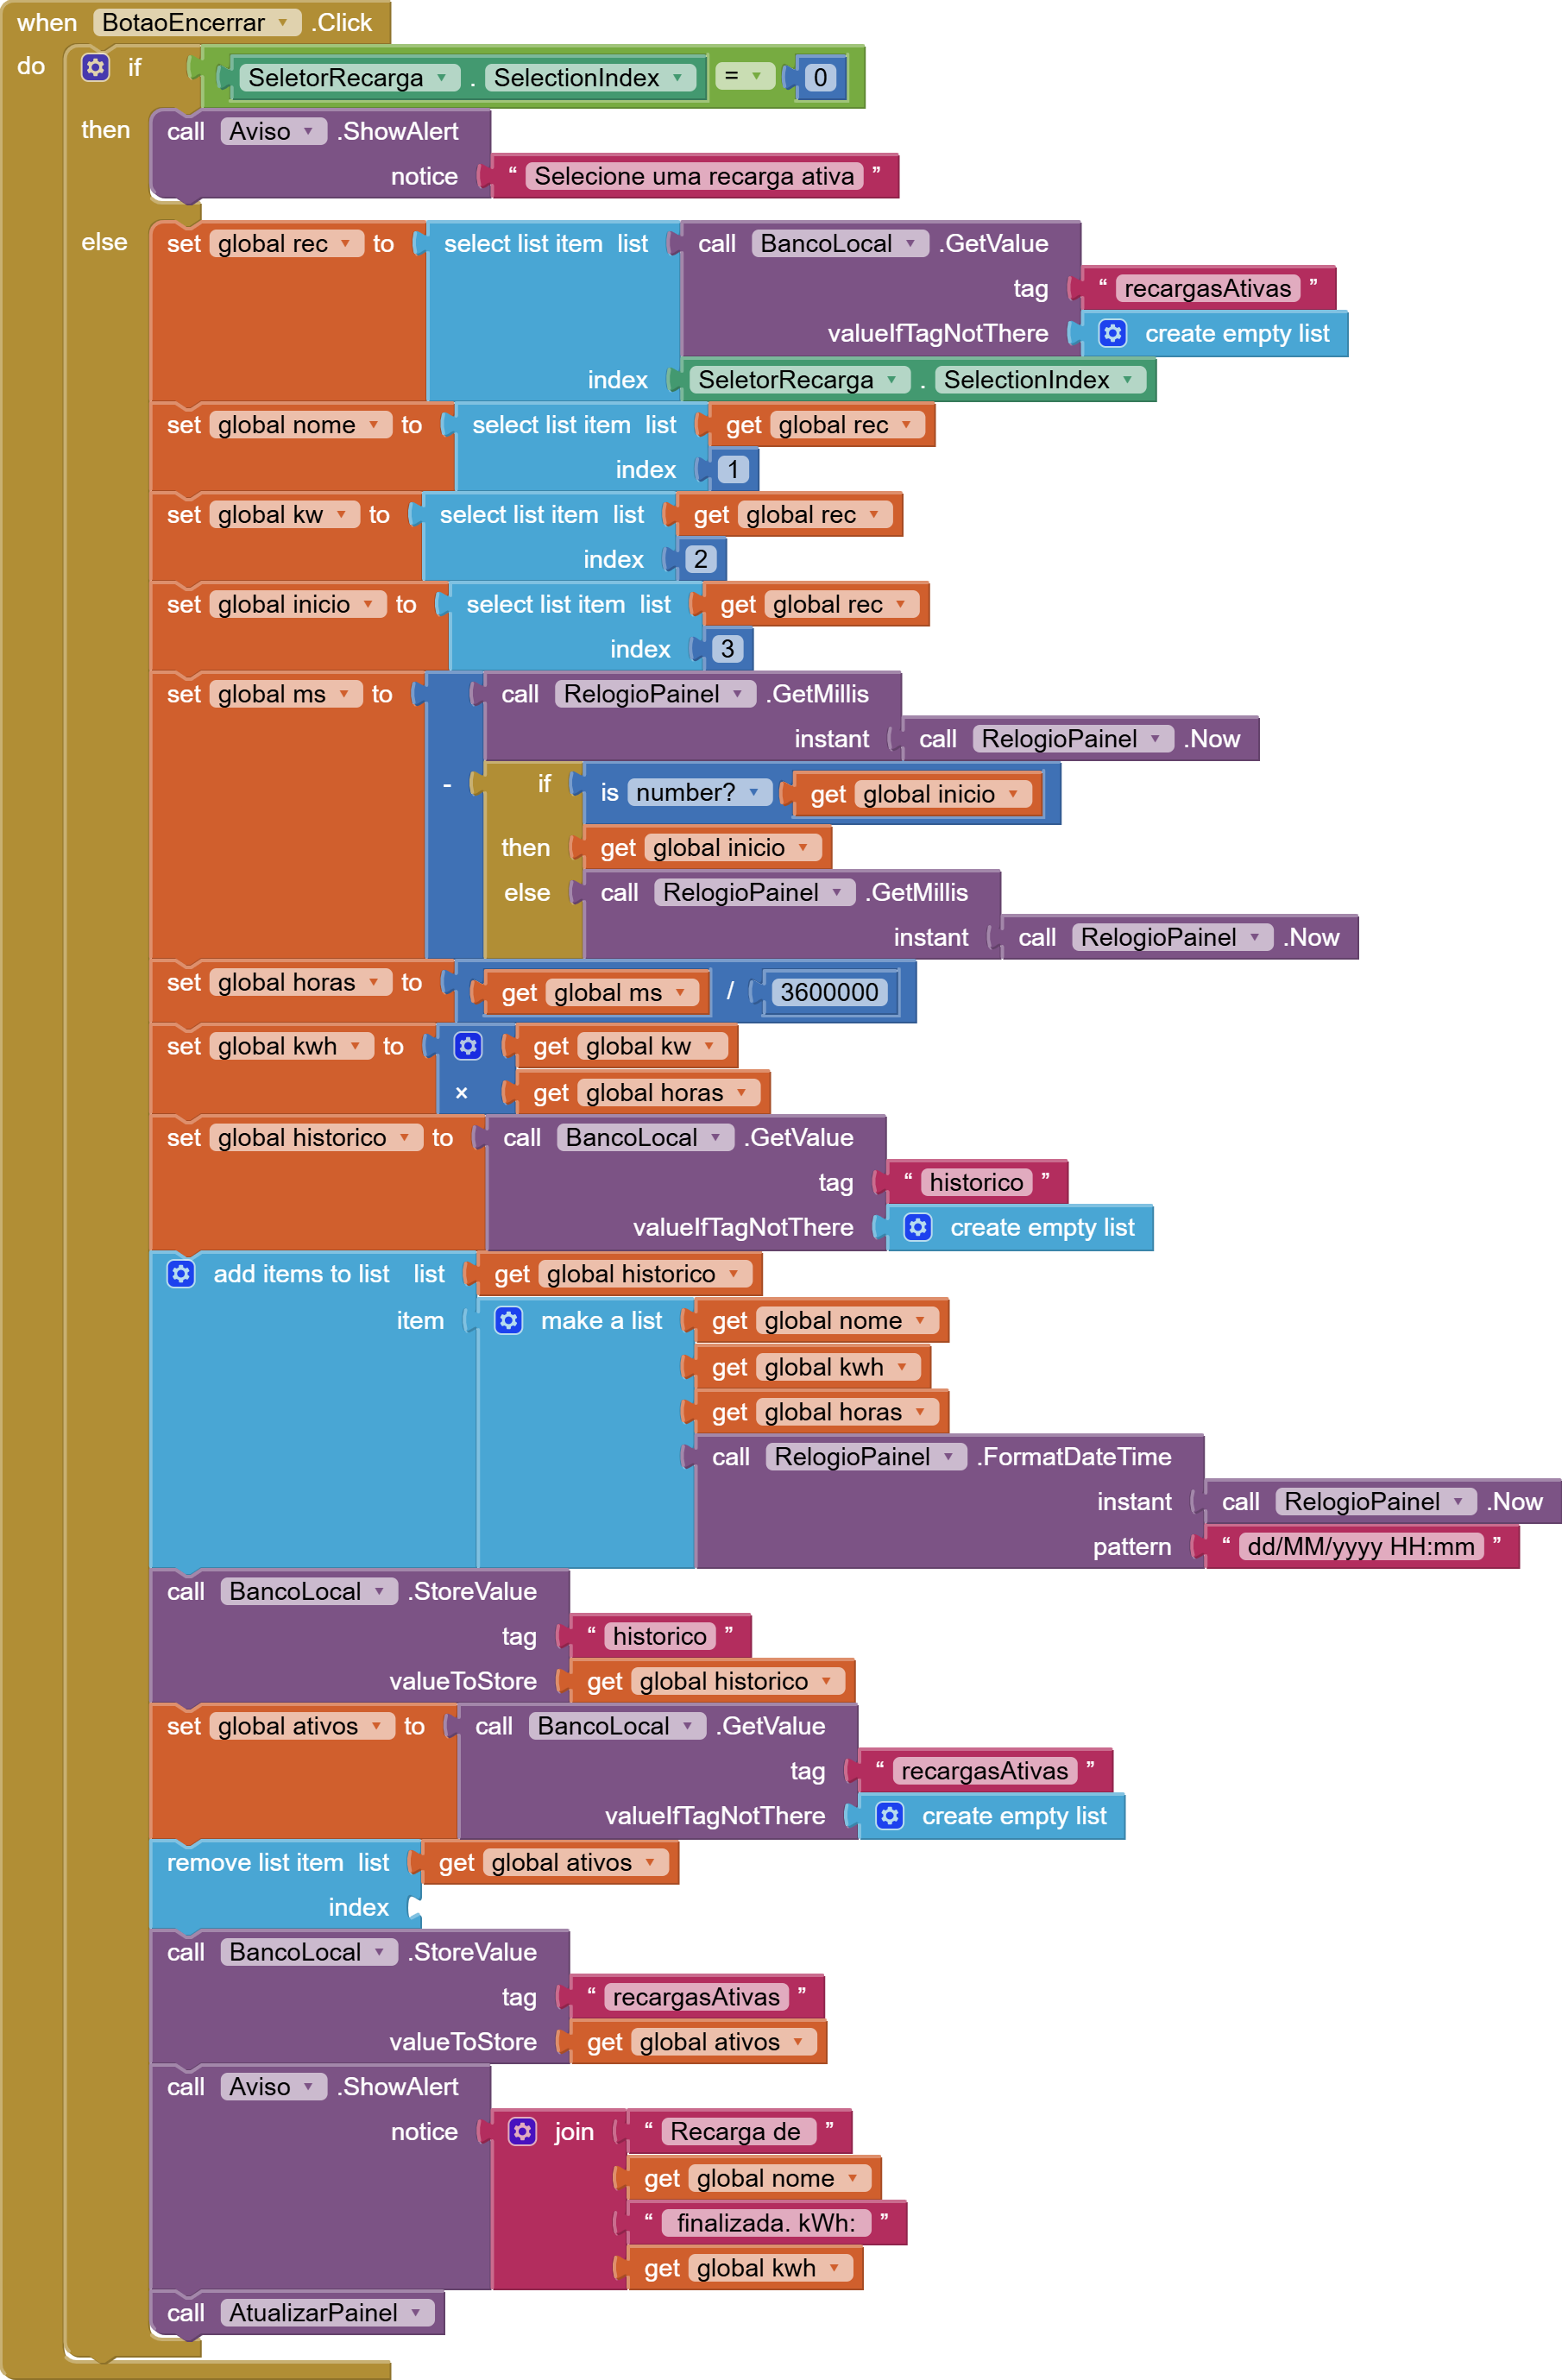
\includegraphics[height=0.80\textheight]{painel-encerrar.png}
\caption{\comp{BotaoEncerrar.Click}. Primeiro verifica se há alguma recarga selecionada.
Havendo, recupera o registro da lista de ativas, calcula a duração pela diferença de
milissegundos, obtém a energia consumida multiplicando potência por horas, acrescenta o
resultado ao histórico no TinyDB, remove a recarga da lista de ativas, confirma ao usuário
e atualiza o painel.}
\end{figure}

O cálculo, em três passos:
\[
\text{ms} = \text{agora} - \text{início}
\qquad
\text{horas} = \frac{\text{ms}}{3\,600\,000}
\qquad
\text{kWh} = \text{kW} \times \text{horas}
\]

Um carregador de 7,2~kW ligado por duas horas e meia consome, portanto, 18~kWh. A distinção
entre as duas unidades é o que torna a cobrança possível: \textbf{kW} é a velocidade com
que a energia é puxada, \textbf{kWh} é a quantidade efetivamente consumida. Só a segunda
vira dinheiro na conta do condomínio.

\subsection{Cadastro: validação encadeada}

\begin{figure}[H]
\centering
\begin{minipage}{0.49\textwidth}
\centering
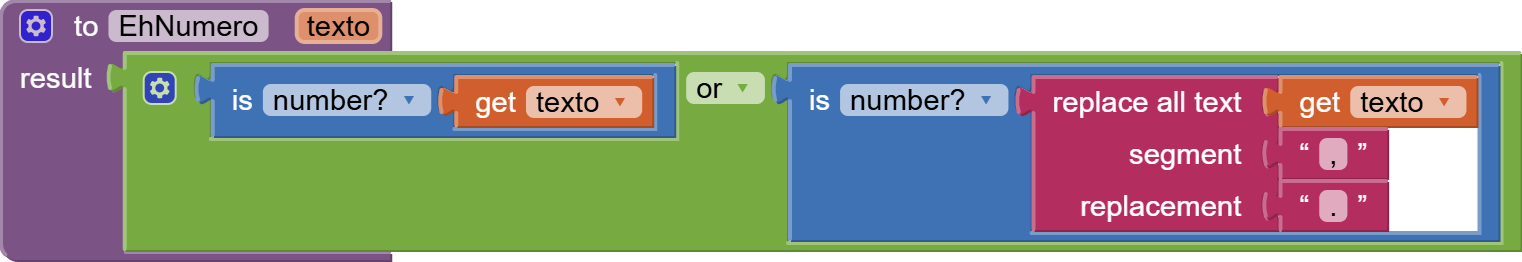
\includegraphics[width=\linewidth]{cadastro-ehnumero.png}
\end{minipage}\hfill
\begin{minipage}{0.49\textwidth}
\centering
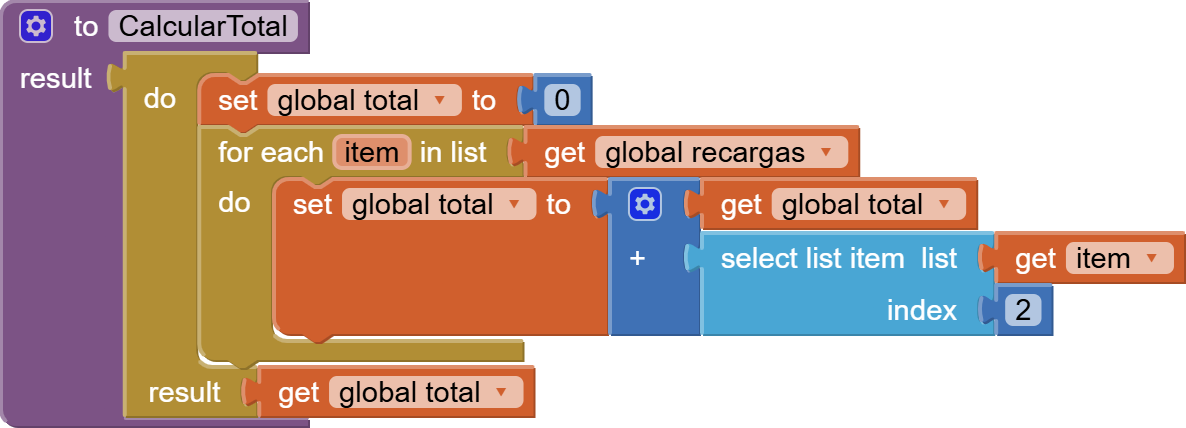
\includegraphics[width=\linewidth]{cadastro-calculartotal.png}
\end{minipage}
\caption{Os dois procedimentos auxiliares do cadastro. \comp{EhNumero} aceita o valor tanto
com ponto quanto com vírgula, testando as duas formas. \comp{CalcularTotal} soma a potência
das recargas já ativas, e é o que permite saber se ainda há capacidade disponível.}
\end{figure}

A Figura~\ref{fig:salvar} mostra a validação encadeada exigida pelo enunciado. São quatro
ramos, avaliados em ordem:

\begin{enumerate}[itemsep=2pt]
\item \textbf{Nome vazio} $\rightarrow$ ``Informe o nome do morador''.
\item \textbf{Potência inválida} --- campo vazio, não numérico, menor que 1 ou maior que o
      limite $\rightarrow$ mensagem dinâmica com a faixa aceita.
\item \textbf{Capacidade insuficiente} --- a soma das recargas ativas com a nova
      ultrapassaria o limite $\rightarrow$ ``Recarga não permitida''.
\item \textbf{Caso contrário} --- monta a lista \comp{[nome, potência, início]}, grava em
      \comp{recargasAtivas} no TinyDB, confirma e fecha a tela.
\end{enumerate}

O terceiro ramo é o que diferencia o aplicativo de um caderno de anotações: ele
\textbf{recusa} uma operação que colocaria a rede em risco, em vez de apenas registrá-la.

\begin{landscape}
\begin{figure}[H]
\centering
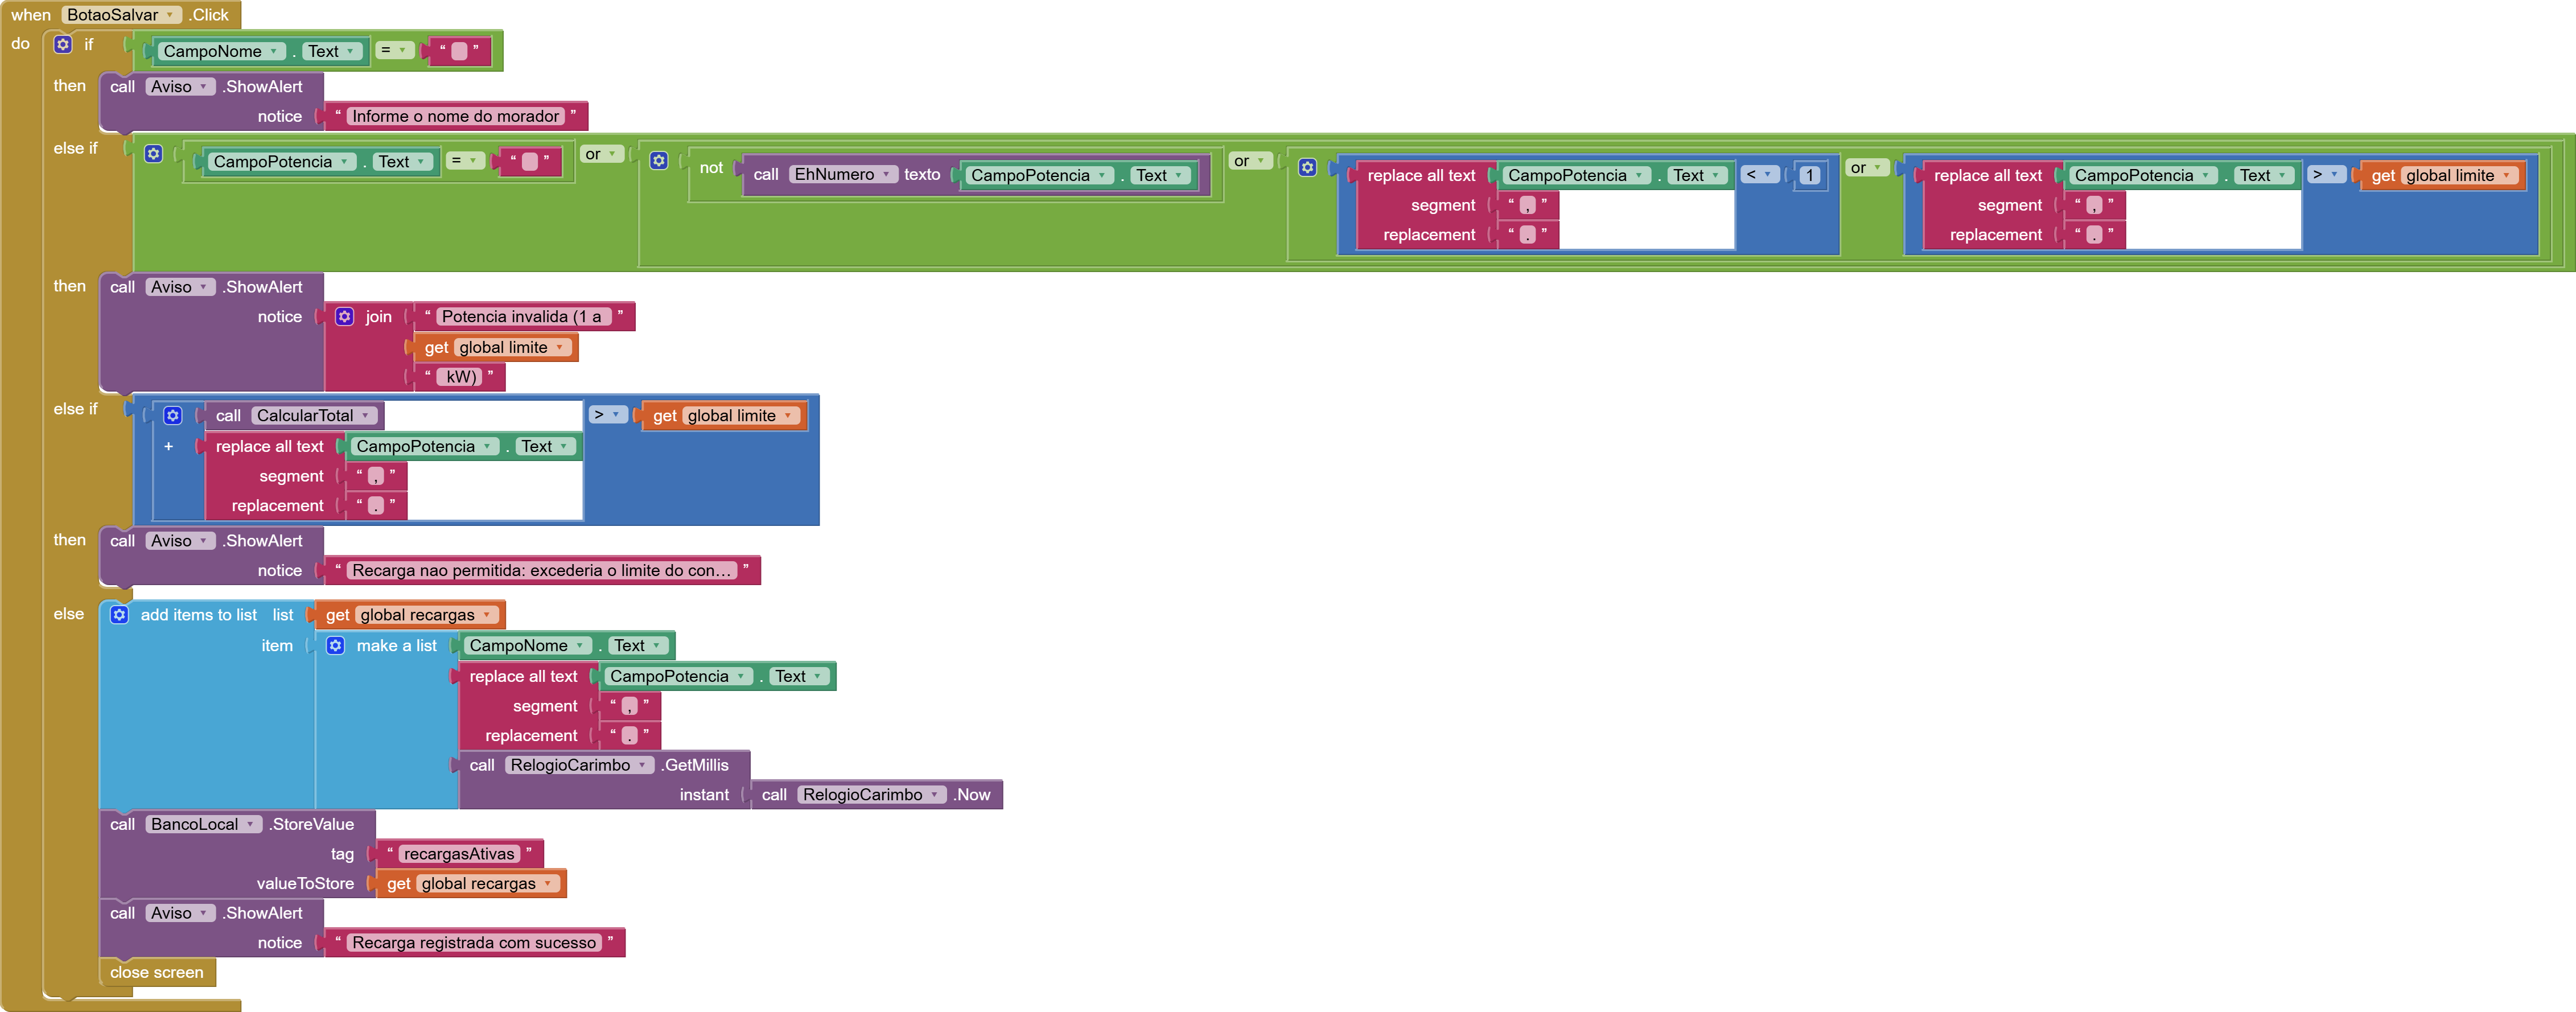
\includegraphics[width=\linewidth]{cadastro-salvar.png}
\caption{\comp{BotaoSalvar.Click} --- a validação encadeada do cadastro. Os três primeiros
ramos rejeitam a entrada com mensagens específicas; o último grava a recarga no TinyDB e
fecha a tela. Página em orientação paisagem por causa da largura do diagrama.}
\label{fig:salvar}
\end{figure}
\end{landscape}

\subsection{Histórico: leitura do TinyDB}

\begin{figure}[H]
\centering
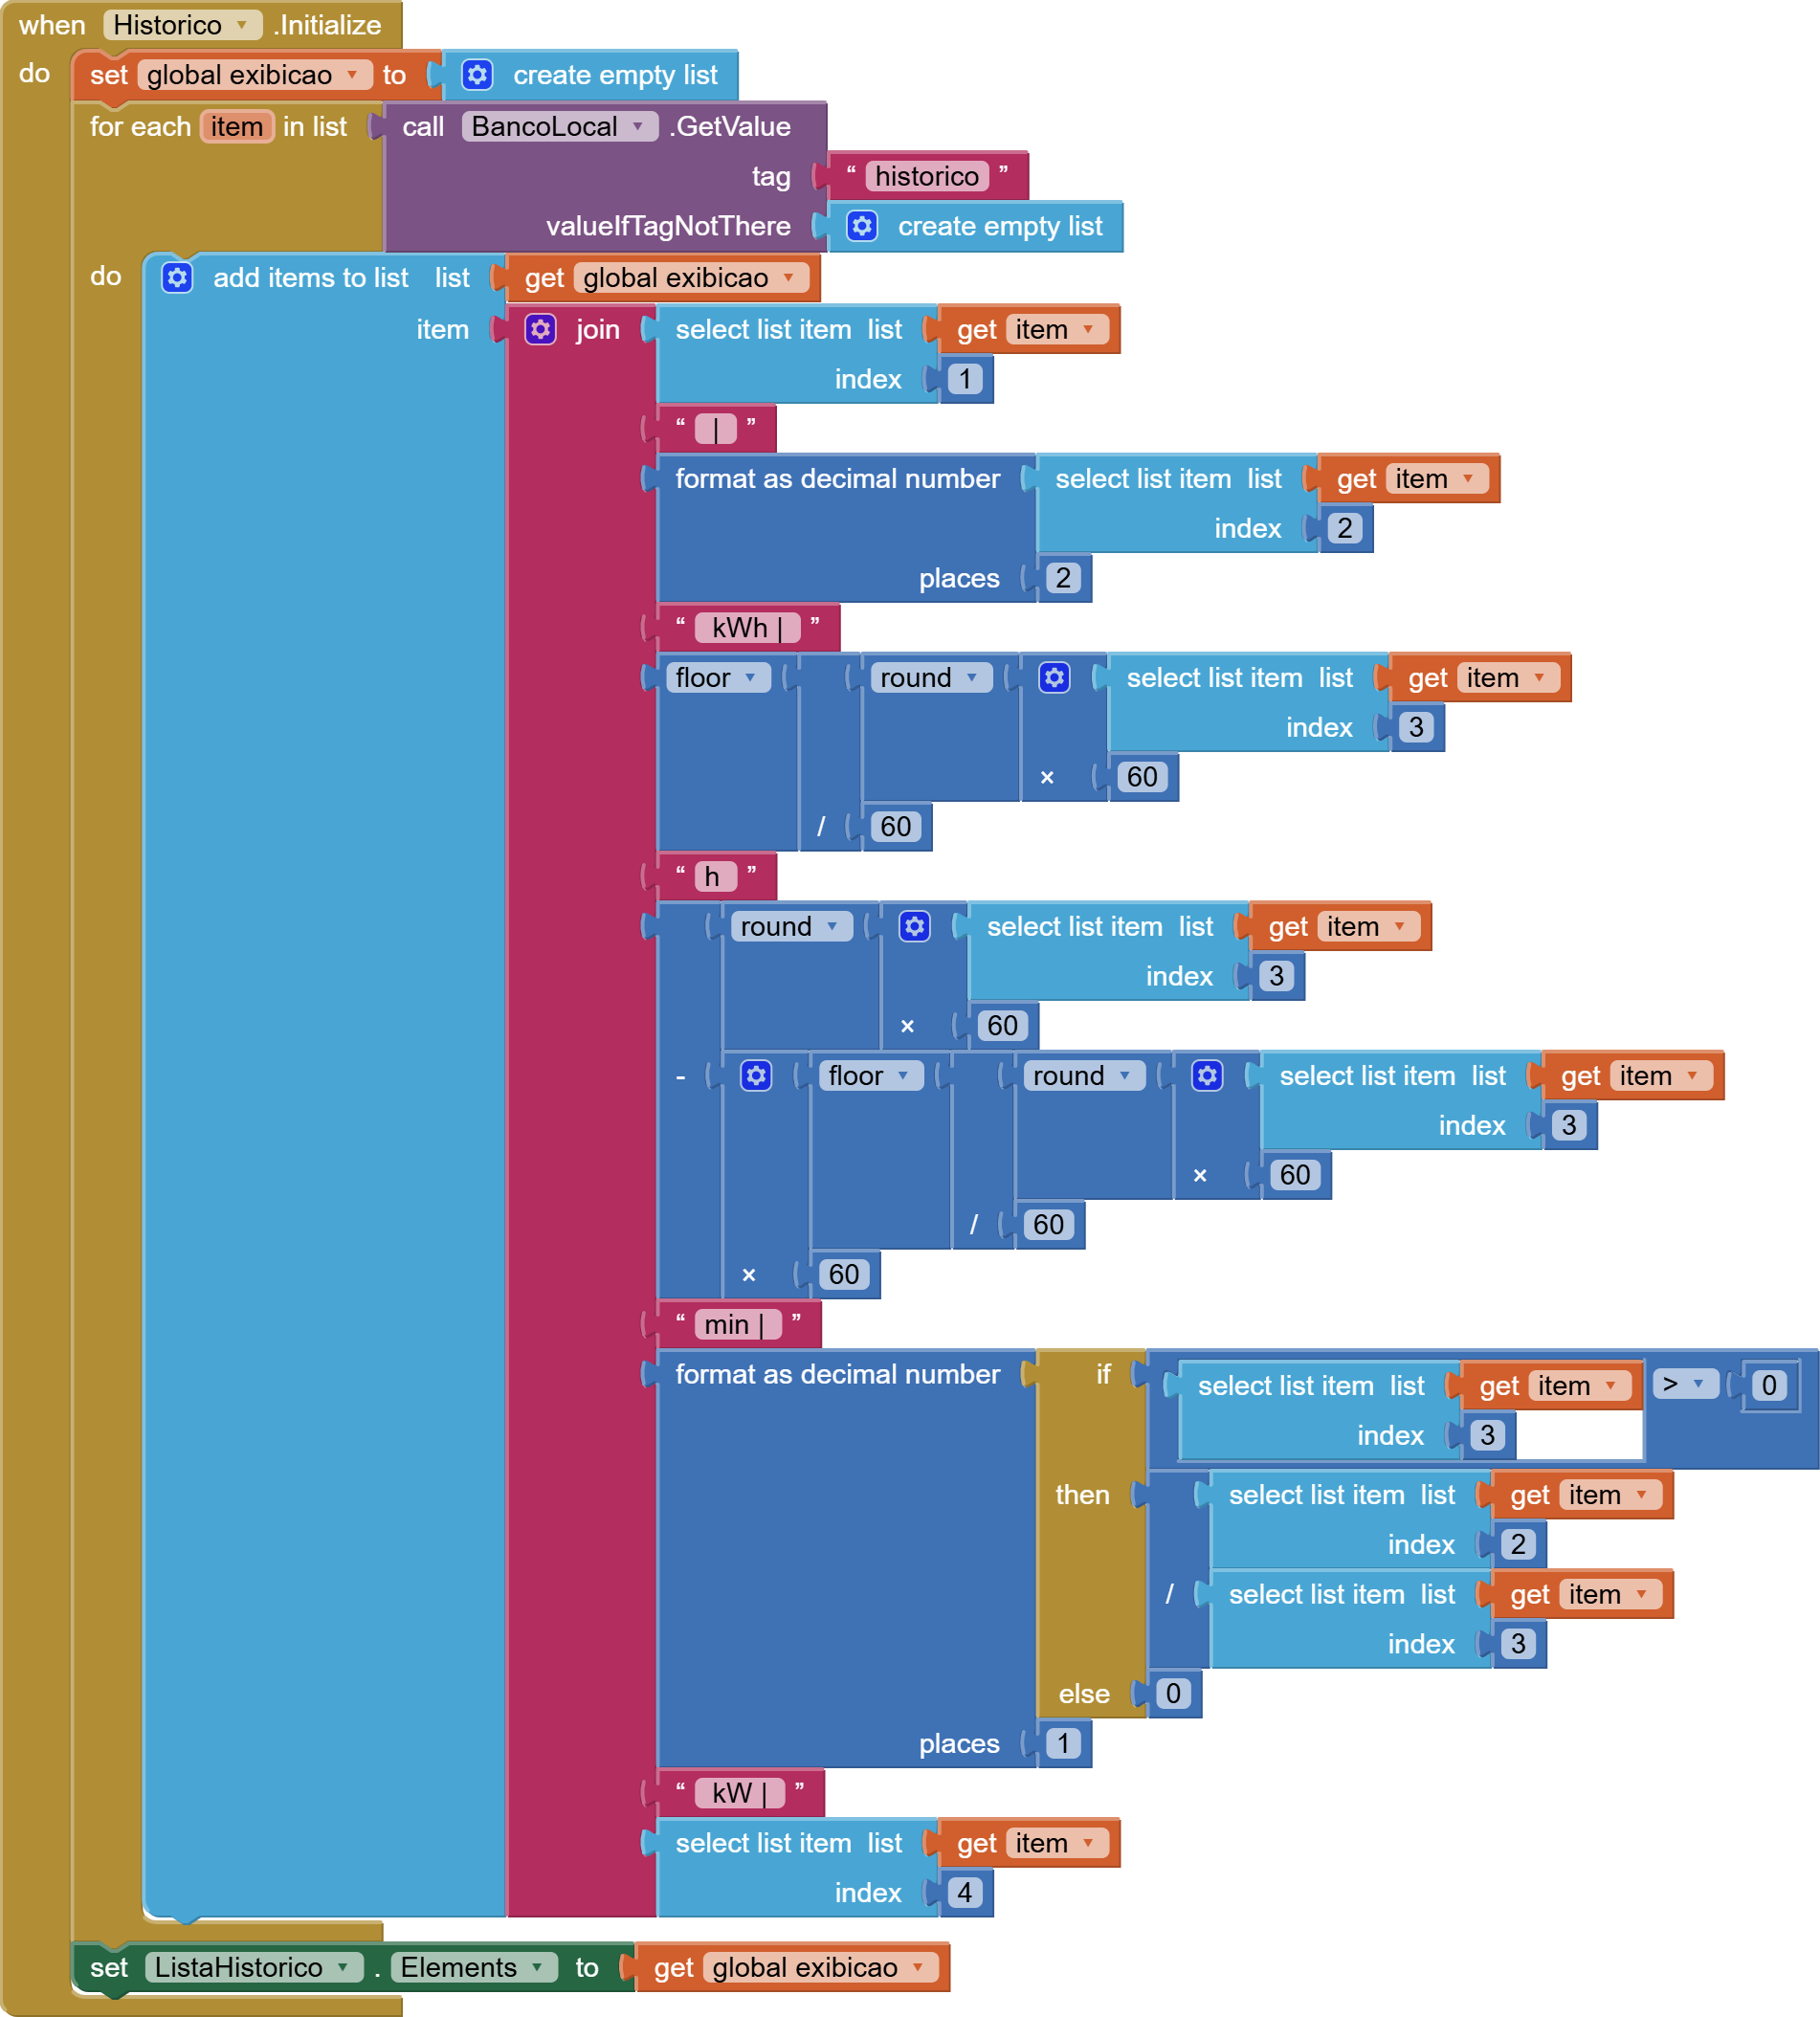
\includegraphics[height=0.72\textheight]{historico-monta-lista.png}
\caption{\comp{Historico.Initialize}. Percorre a lista \comp{historico} do TinyDB e monta,
para cada registro, uma linha de texto formatada: energia com duas casas decimais, duração
convertida de horas decimais para horas e minutos, e potência derivada da razão entre
energia e duração. O resultado alimenta a \comp{ListaHistorico}.}
\end{figure}

\begin{figure}[H]
\centering
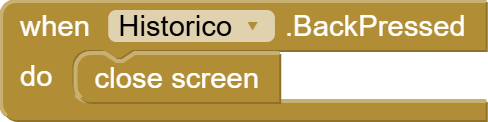
\includegraphics[width=0.55\textwidth]{historico-voltar.png}
\caption{\comp{Historico.BackPressed}. Trata o botão físico de voltar do aparelho, fechando
a tela pelo mesmo caminho do botão ``Voltar''. Sem esse tratamento, o comportamento fica a
cargo do sistema operacional.}
\end{figure}

% ===========================================================================
\section{Proposta de valor}

Para um condomínio antigo, a solução tecnicamente correta é reforçar a rede elétrica. Isso
custa caro, depende de assembleia, de orçamento e de rateio --- e os moradores sem veículo
elétrico têm motivo para votar contra.

O Torre EV não substitui essa obra. Ele resolve outro problema, que existe \textbf{hoje} e
não tem solução de custo zero: dar ao síndico a informação que falta para conviver com o
limite atual sem derrubar o prédio.

\begin{table}[H]
\centering
\small
\begin{tabular}{@{}p{6.4cm}p{6.4cm}@{}}
\toprule
\textbf{Antes} & \textbf{Depois} \\
\midrule
Ninguém sabe quanto está sendo puxado da rede &
Painel mostra a carga total em tempo real \\
\addlinespace
Descobre-se o excesso quando o disjuntor cai &
Aviso sonoro aos 80\% do limite, antes do estrago \\
\addlinespace
Recarga que estoura a rede é ligada assim mesmo &
O cadastro é recusado com a justificativa \\
\addlinespace
Consumo diluído na conta da área comum &
kWh registrado no nome de cada morador \\
\bottomrule
\end{tabular}
\caption{O que muda com a adoção do aplicativo.}
\end{table}

Três características sustentam a adequação ao contexto de um prédio antigo:

\begin{itemize}[itemsep=3pt]
\item \textbf{Custo zero de infraestrutura.} Roda no celular que o síndico já tem. Não
      exige sensor, medidor, obra ou aprovação em assembleia.
\item \textbf{Limite configurável.} A capacidade disponível varia de prédio para prédio e
      pode mudar após uma reforma. O síndico ajusta na própria tela, sem alterar o
      aplicativo.
\item \textbf{Dados locais.} Nenhuma dependência de internet, servidor ou conta em
      serviço externo --- o que também elimina qualquer questão sobre dados pessoais dos
      moradores saindo do prédio.
\end{itemize}

% ===========================================================================
\section{Limitações conhecidas}

Registrar os limites faz parte da honestidade técnica do trabalho:

\begin{itemize}[itemsep=3pt]
\item \textbf{O aplicativo não mede energia.} Os dados são informados pelo síndico. Se ele
      esquecer de dar baixa, o painel continuará considerando a recarga ativa.
\item \textbf{Não atua sobre o carregador.} Alerta e recusa cadastro, mas não interrompe
      fisicamente nenhuma recarga.
\item \textbf{Uso individual.} Os dados ficam no aparelho do síndico. Troca de celular ou
      alternância entre dois síndicos exigiria sincronização, que está fora do escopo.
\item \textbf{Não emite cobrança.} O sistema apura o consumo por morador; converter isso em
      rateio continua sendo trabalho da administração.
\item \textbf{O histórico só recebe registro no encerramento.} Salvar uma recarga nova a
      coloca entre as ativas; ela só aparece no histórico depois de encerrada.
\end{itemize}

\end{document}
